\chapter{Protocollo SSL (\emph{Secure Socket Layer})}
\section{Introduzione}
\[\boxed{\text{L'utente $U$ desidera accedere via Internet a un servizio offerto dal sistema $S$.}}\]
SSL (\emph{Secure Socket Layer}) è alla base dei protocolli più diffusi nelle comunicazioni sicure. Lo portiamo come esempio perchè combina molte cose viste durante il corso. 
\begin{itemize}
	\item Oggi non si utilizza la versione che introdurremo, ma il TLS (\emph{Transport Layer Security}, variante con qualche modifica).
	\item Garantisce \textbf{confidenzialità} e \textbf{affidabilità} delle comunicazioni su internet proteggendole da intrusioni, modifiche e falsificazioni.
	\item Sviluppato inizialmente da \textit{Netscape} per mettere in sicurezza HTTP, è progettato in modo da permettere la comunicazione tra computer che non conoscono le reciproche funzionalità.
	\item Garantisce la confidenzialità tramite l'uso di un sistema ibrido: 
	\begin{itemize}
		\item cifrario asimmetrico per la costruzione e lo scambio delle chiavi di sessione;
		\item cifrario simmetrico per la cifratura delle comunicazioni.
	\end{itemize}
	\item Garantisce l'autenticazione dei messaggi accertando l'identità dei due partner attraverso sia un cifrario asimmetrico che tramite certificati digitali con un MAC (\emph{Message Autentication Code}, che usa una funzione hash one way crittograficamente sicuro).
	\item Si trova tra il TCP (trasporto) e HTTP (applicazione) ma è totalmente indipendente dal protocollo applicativo sovrastante (HTTPS = HTTP su SSL).
\end{itemize}

\section{Livelli in cui SSL è organizzato}
SSL è organizzato in:
\begin{itemize}
	\item \textbf{SSL record}.
	
	Livello più basso, connesso direttamente al protocollo di trasporto. Ha l'obiettivo di incapsulare i dati spediti dai livelli superiori assicurando confidenzialità ed integrità.
	
	\item \textbf{SSL handshake}.
	
	Instaura e mantiene i parametri poi usati da SSL record. Si permette a utente e sistema di:
	\begin{itemize}
		\item autenticarsi;
		\item negoziare gli algoritmi di cifratura e firma;
		\item stabilire le chiavi per i signoli algoritmi crittografici e per il MAC.
	\end{itemize}
	Il tutto permette di creare un canale di comunicazione sicuro, affidabile e autenticato tra utente e sistema, all'interno del quale SSL Record fa viaggiare i messaggi. Abbiamo uno scambio di messaggi preliminare (\emph{handshake}) per la creazione del canale sicuro: attraverso questi messaggi il sistema $S$ e l'utente $U$
	\begin{itemize}
		\item si identificano a vicenda, e
		\item cooperano nella costruzione delle chiavi segrete da impiegare nelle comunicazioni successive.
	\end{itemize}
\end{itemize}
Vediamo singolarmente le fasi.

\section{Fasi in SSL handshake}
\subsection{Messaggio \emph{client hello} inviato dall'utente $U$}
L'utente $U$ invia al sistema $S$ un messaggio con il quale:
\begin{itemize}
	\item si richiede la creazione di una connessione SSL;
	\item specifica i cifrari e meccanismi che supporta e le prestazioni di sicurezza richieste;
	\item invia una sequenza di byte casuali.
\end{itemize} 
Tutto questo è mandato in chiaro!

\paragraph{Esempio} Un esempio di \emph{client hello} è la \emph{cypher suite}. 
\[\boxed{\text{SSL\_RSA\_WITH\_AES\_CBC\_SHA1}}\]
Vuole utilizzare i seguenti cifrari:
\begin{itemize}
    \item \textbf{RSA} per lo scambio delle chiavi di sessione;
    \item \textbf{AES} come cifratura simmetrica;
    \item \textbf{CBC} come composizione dei blocchi;
    \item \textbf{SHA1} come funzione hash per il MAC.
\end{itemize}
Questo è un esempio di \emph{cipher suite}. Il sistema risponderà nella fase successiva: \emph{server hello}.

\subsection{Messaggio \emph{server hello} inviato dal server $S$}
Il sistema $S$ riceve il messaggio dell'utente $U$.
\begin{itemize}
	\item Seleziona una cipher suite che anche lui supporta (cerca di soddisfare le richieste dell'utente $U$)
	\item Invia un messaggio all'utente $U$ dove specifica la sua scelta.
	\item Appende dei byte casuali alla risposta. 
\end{itemize}
Anche questo è mandato in chiaro!

\paragraph{NB} Se $U$ non riceve il \emph{server hello} allora interromperà la comunicazione.

\subsection{Autenticazione (creazione certificato da parte del sistema $S$)}
Il sistema $S$ si autentica con $U$ inviandogli il proprio certificato digitale (e gli eventuali altri certificati fino al primo nodo comune nella catena delle CA).

\paragraph{NB} Se i servizi offerti da $S$ devono essere protetti negli accessi anche $S$ può richiedere a $U$ di autenticarsi inviando il suo certificato digitale. Avviene raramente in quanto la maggior parte degli utenti non ha un proprio certificato e in genere ci si accerta dell'identità di un utente in un secondo modo (autenticazione sul sito web ad esempio).

\subsection{Messaggio \emph{server hello done}}
Messaggio con il quale il server $S$ sancisce la fine degli accordi sulla cipher suite ed i parametri crittografici associati.

\subsection{Controllo del certificato da parte dell'utente $U$}
L'utente $U$ accerta l'autenticità del certificato ricevuto dal sistema $S$ tramite la data, tramite la CA che lo ha firmato, ecc. Estrae la chiave pubblica dal certificato. L'utente $U$:
\begin{itemize}
	\item costruisce il \emph{pre-master secret} costituito da una nuova sequenza casuale di byte;
	\item lo cifra con la chiave pubblica estratta dal certificato.
	\item spedisce il crittogramma al sistema $S$.
\end{itemize}


\subsection{Costruzione del \emph{master secret} presso l'utente $U$}
Sempre l'utente $U$ costruisce il \emph{master secret} partendo da:
\begin{itemize}
	\item il \emph{pre-master secret} (cifrato con RSA, si usa la chiave pubblica presente nel certificato di $S$);
	\item i byte casuali di \emph{client hello} e \emph{server hello} (\emph{client hello} lo ha di suo, mentre \emph{server hello} è stato inviato dal server).
\end{itemize} 
Applica a tutte queste sequenze delle funzioni hash one-way secondo una combinazione opportuna. Il nuovo valore ottenuto è il \emph{master secret}.

\subsection{Ricostruzione del \emph{master secret} presso il server $S$}
Anche il sistema $S$ si calcola localmente il master secret. Può farlo perchè possiede:
\begin{itemize}
	\item il \emph{pre-master secret}, appena ricevuto dall'utente $U$ e decriptato con la sua chiave privata
	\item i byte casuali di \emph{client hello} e \emph{server hello} (\emph{client hello} lo ha ricevuto dall'utente $U$, mentre \emph{server hello} lo ha di suo)
\end{itemize}
Entrambi gli utenti hanno il \emph{master secret}!

\subsubsection{Extra: Autenticazione dell'utente $U$ (se richiesto certificato a $U$)}
\begin{itemize}
	\item Se all'utente $U$ è richiesto un certificato ed egli non lo possiede il sistema $S$ interrompe l'esecuzione del protocollo.
	\item Altrimenti $U$ invia il proprio certificato allegando \emph{master secret} e la SSL-history (tutti i messaggi scambiati fino a quel momento) firmate con la sua chiave privata.
	\item Il sistema $S$ controlla certificato ed SSL-history: \textbf{nel caso in cui emergano ambiguità la comunicazione viene interrotta}.
\end{itemize}


\subsection{Messaggio \emph{finished} inviato sia dall'utente che dal server}
E' il primo messaggio protetto da \emph{master secret} e \emph{cipher suite} accordati. Il messaggio è costruito dall'utente $U$ e inviato al sistema $S$, poi costruito dal sistema $S$ ed inviato all'utente $U$. Il messaggio ha la stessa struttura ma cambiano i dati (la history).
\paragraph{Costruzione del messaggio} La costruzione avviene:
\begin{itemize}
    \item concatenazione di master secret, messaggi di handshake scambiati fino al momento attuale, e l'identità del mittente ($U$ o $S$);
    \item la stringa ottenuta viene trasformata applicando funzioni hash, sia con SHA-1 che con MD5. 
\end{itemize}
I due messaggi (quello trasmesso dall'utente $U$ e quello successivamente trasmesso dal server $S$) sono diversi in quanto il sistema $S$ aggiunge anche la \emph{finished} ricevuta da $U$ (che adesso fa parte della history). Non sono ovviamente invertibili perché costruiti tramite hash.
\paragraph{Uso del master secret} Il master secret viene usato per creare le chiavi:
\begin{itemize}
    \item chiave segreta per il cifrario simmetrico
    \item chiave per l'autenticazione del messaggio (MAC)
    \item \textit{initialization vector} per il CBC
\end{itemize}
Le terne di chiavi di $U$ ed $S$ sono diverse tra loro ma note ad entrambi, ciascuno usa la propria, quindi aumenta la sicurezza.

\section{SSL Record}
Successivamente i parametri vengono passati al SSL Record che si occupa del vero e proprio dialogo dei dati suddividendo i dati in blocchi, aggiungendo un MAC ad ogni blocco, cifrato con il protocollo simmetrico scelto e trasmesso al protocollo di trasporto sottostante. Il destinatario esegue il contrario.


\section{Sicurezza di SSL}
\begin{itemize}
	\item Nei passi di \textit{hello} i due partner creano e si inviano sequenze casuali per costruire la master secret, questo risulta in chiavi diverse ogni volta. Un crittoanalista non può riutilizzare i messaggi catturati sul canale per sostituirli a S successivamente.
	\item L'SSL record successivamente numera ogni blocco in maniera incrementale e lo autentica tramite MAC.
	Un blocco non può essere modificato in quanto il MAC è hash di:
	\begin{itemize}
		\item contenuto
		\item numero sequenziale del blocco
		\item chiave del MAC
		\item altre stringhe note e fissate a priori
	\end{itemize}
\item MAC e messaggio sono cifrati quindi prima di poterli alterare va forzato il cifrario.

\item Non si possono eseguire man-in-the-middle in quanto si usano i certificati.

\item Il pre-master secret è inviato cifrato con chiave pubblica quindi è sicuro.

\item Quindi solo $S$, proprietario della chiave privata associata al certificato può recuperare la pre-master key e quindi entrare in comunicazione con $U$.

\item Anche $U$ può essere autenticato se necessario.
Se è richiesto ma non avviene la comunicazione salta.
L'opzionalità di questa autenticazione ha reso usato questo protocollo in quanto può essere autenticato in altri modi, magari lato applicazione.

\item Le sequenze sono generate a partire da byte casuali quindi una sua predicibilità metterebbe a rischio tutto.

\item Il messaggio finished contiene tutta la history e quidi permette un ulteriore controllo finale. E' sicuro almeno quanto il cifrario più debole della cipher suite, ma non ci sono cifrari deboli lasciati dentro.
\end{itemize}






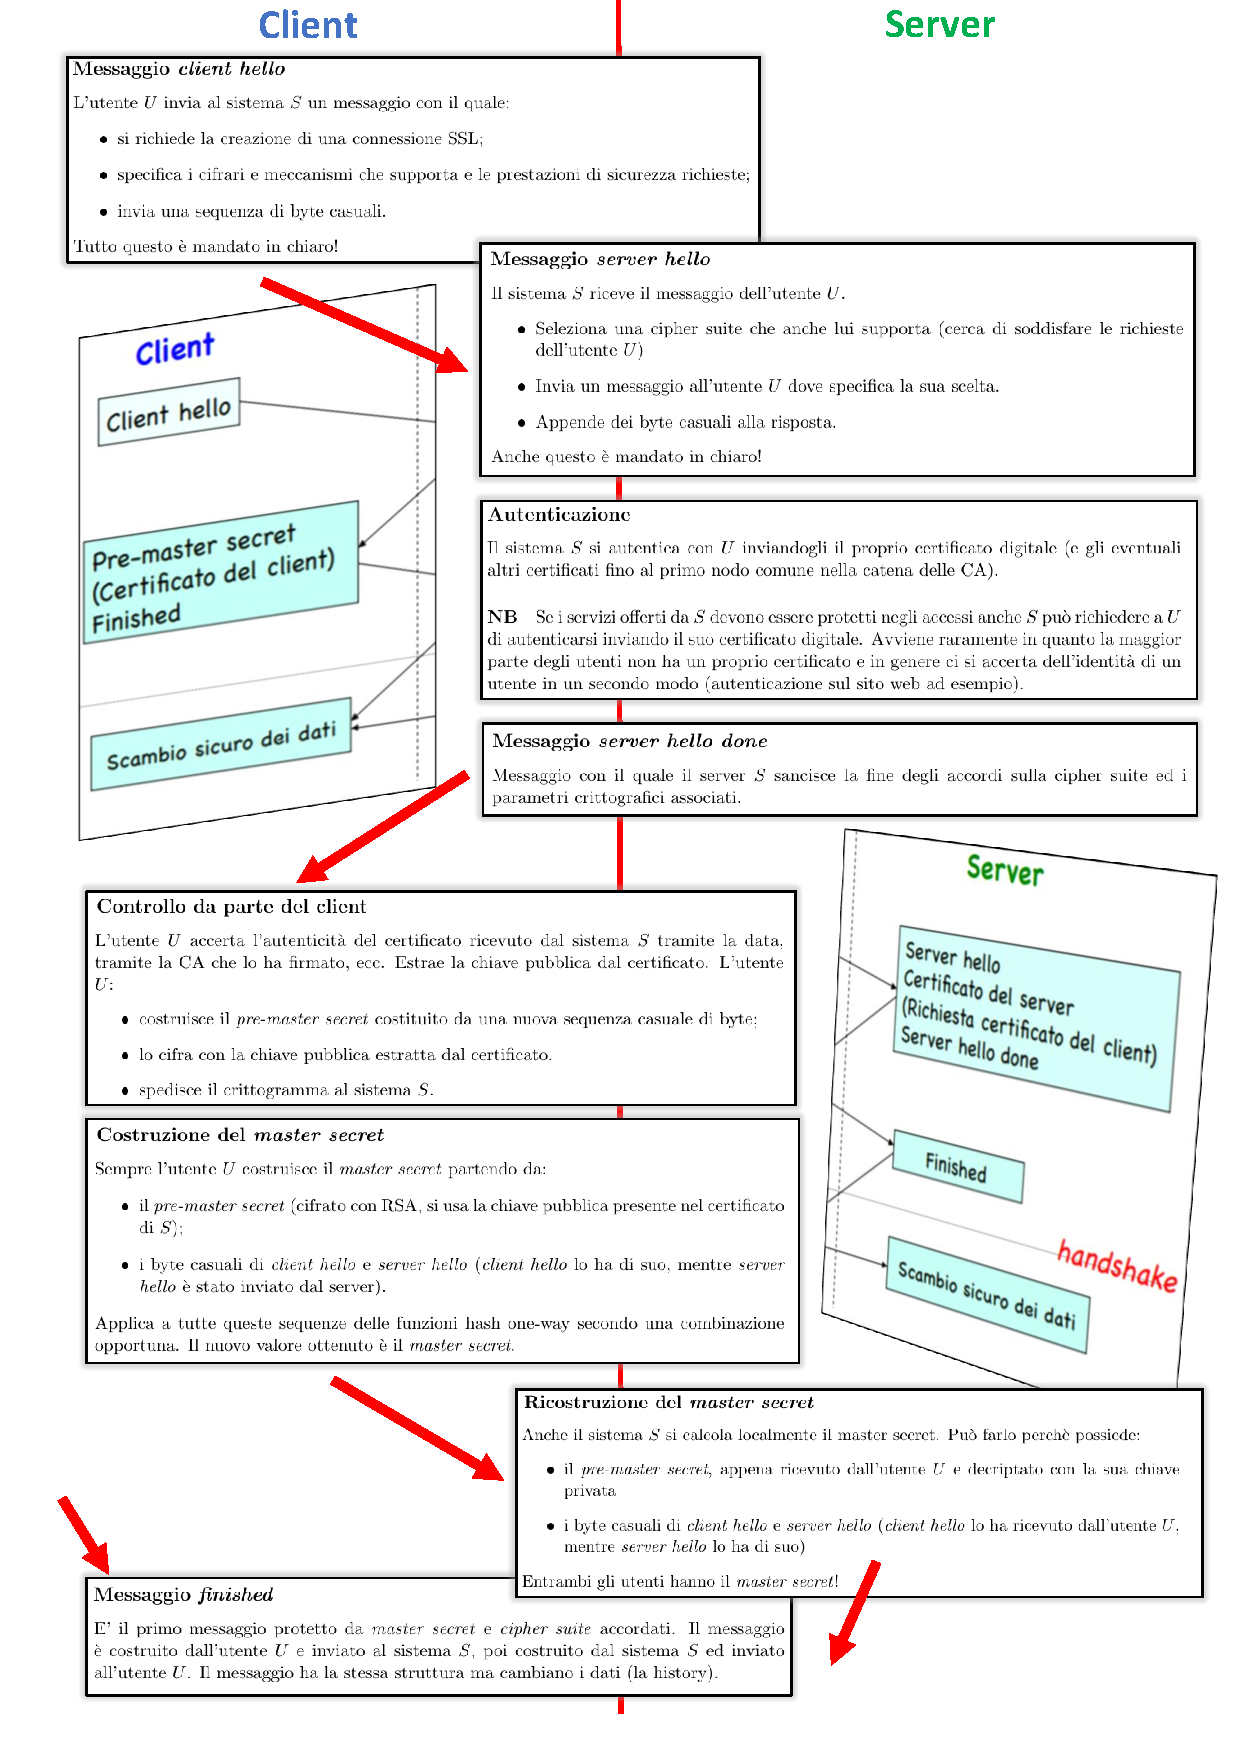
\includepdf[pagecommand={\thispagestyle{plain}},scale=0.84,pages=-]{pdf/schemassl}